\documentclass[margin,line]{res}
\usepackage[utf8]{inputenc}
\usepackage{multirow}
\usepackage{graphicx}

\oddsidemargin -.5in
\evensidemargin -.5in
\textwidth=6.0in
\itemsep=0in
\parsep=0in

\newenvironment{list1}{
  \begin{list}{\ding{113}}{%
      \setlength{\itemsep}{0in}
      \setlength{\parsep}{0in} \setlength{\parskip}{0in}
      \setlength{\topsep}{0in} \setlength{\partopsep}{0in} 
      \setlength{\leftmargin}{0.17in}}}{\end{list}}
\newenvironment{list2}{
  \begin{list}{$\bullet$}{%
      \setlength{\itemsep}{0in}
      \setlength{\parsep}{0in} \setlength{\parskip}{0in}
      \setlength{\topsep}{0in} \setlength{\partopsep}{0in} 
      \setlength{\leftmargin}{0.2in}}}{\end{list}}


\begin{document}

\name{Óscar Andrés Nájera Ocampo}

\begin{resume}

\section{\sc Contact Information}
  \begin{tabular}{@{}p{2in}p{2.5in}p{3cm} }
    {\it Work Address:}		& {\it work:}  +41 44 633 06 41 &
      \multirow{4}{*}{ 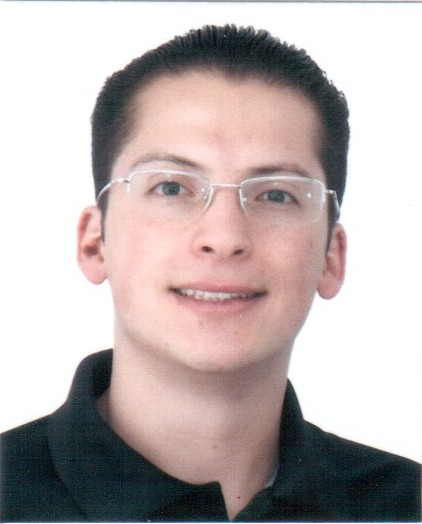
\includegraphics[width=3cm,bb=0 0 101 126]{./foto2012.jpg}}\\

    HIT G 23.6			& {\it mobile:} +41 78 729 35 96 \\
    Wolfgang-Pauli Str. 27	& {\it e-mail:}  najera.oscar@ifb.baug.ethz.ch\\
    8093 - Zürich, Schweiz	& {\it www:} http://titan-c.github.com
  \end{tabular}\vspace{0.5cm}

\section{\sc Personal Information}
 \begin{tabular}{ll}
  {\it Family Name:} Nájera Ocampo & {\it Date of Birth:} 13 April 1988\\
  {\it Given Name:} Óscar Andrés   & {\it Gender:} Male\\
  {\it Nationality:} Ecuadorian    & %{\it Marital status:} Single
 \end{tabular}

\section{\sc Research Interests}
  Condensed Matter, Solid State Physics, Statistical Mechanics, Mathematical \& Theoretical Physics, Scientific Programming \& computational systems analysis

\section{\sc Education}
%   {\bf Universidad Central del Ecuador}, Quito, Ecuador\\
%   \vspace{-.1in}
%   \begin{list1}
%     \item[] Master in Mathematics \hfill {\bf Nov. 2012 - present}
%     \item[] Joint Master program with {\it Escuela Politécnica Nacional} \& {\it Universidad
%     San Francisco de Quito} in Quito - Ecuador and {\it Université Jean Monnet} in
%     Saint-Etienne - France
%   \end{list1}

  {\bf Eidgenössische Technische Hochschule(ETH)}, Zurich, Switzerland\\
  \vspace{-.1in}
  \begin{list1}
    \item[] Doctoral Student \hfill {\bf Apr. 2012 - present}\\
  \end{list1}


  {\bf Escuela Politécnica Nacional}, Quito, Ecuador\\
  \vspace{-.1in}
  \begin{list1}
    \item[] Physics Diploma \hfill {\bf Oct. 2006 - Sept. 2012}\\
    \begin{list2}
    \vspace{-.1in}
      \item Thesis Topic:  ``Estimation, by computer simulation, of the exchange
	energy dispersion between polar nano-regions in $Pb_xBi_4Ti_{3+x}O_{12+3x}; x=\{2,3\}$
	relaxor ferroelectrics''
      \item Advisor: Dr. Luis Lascano
      \item Written in: Spanish
      \item Coursework grades: 8.2/10 | Written thesis: 9.8/10 | Oral examination: 10/10
    \end{list2}
  \end{list1}

  {\bf German School}, Quito, Ecuador\\
  \vspace{-.1in}
  \begin{list1}
    \item[] German Abitur \hfill {\bf May 2006}
    \item[] Ecuadorian High School Diploma \hfill {\bf June 2005}
  \end{list1}

\section{\sc Honors and Awards}
  Danced for Ecuador in WDSF World DanceSport Championship Standard, Australia \hfill {\bf 2012}\\
  Physics Olympiad $1^{st}$ place, Escuela Politécnica Nacional, Ecuador \hfill {\bf 2010}\\
  Bronze Medal for Academic performance, German School Quito, Ecuador \hfill {\bf 2005}\\
  PAD Preisträger, Kultusminister Konferenz, Germany \hfill {\bf 2003}

\section{\sc Academic Experience}
  {\bf Universidad Central del Ecuador}, Quito, Ecuador
  \begin{list1}
    \item[] {\em Trainee in the Molecular Symmetries and Quantum Chemistry Group} \hfill {\bf Oct. 2012 - Mar. 2013}
  \end{list1}

  {\bf Escuela Politécnica Nacional}, Quito, Ecuador
  \begin{list1}
   \item[] {\em Student} \hfill {\bf Oct. 2006 - Sept. 2012}\\
    Includes research and coursework\\
   \item[] {\em Laboratory and teacher's Assistant} \hfill {\bf Aug. 2011 - June 2012}\\
    Responsible of Experimental Physics laboratory in subjects
    like Newtonian Mechanics, Electromagnetism and Optics.
    Shared responsibility for lectures, homework assignments and grades in this subjects.\\
   \item[] {\em Teacher's Assistant} \hfill {\bf Sept. 2010 - Feb. 2011}\\
    Support students in single- \& multi-variable Calculus, and Real Analysis through
    exercise sessions and solutions of exams.
  \end{list1}

  {\bf International Center for Theoretical Physics}, Trieste, Italy
  \begin{list1}
    \item[] {\em Invited Student} \hfill {\bf Mar. 11 - 22, 2013} \\
    Participation at the {\em ``Workshop on Computer Programming and Advanced Tools for Scientific
    Research Work''} SMR 2503
    \item[] {\em Invited Student} \hfill {\bf Feb. 20 - Mar. 2, 2012} \\
    Participation and presentation of research work at the {\em ``Advanced School on Scientific
    Software Development''} SMR 2330
  \end{list1}

\section{\sc Conference Presentations}
  {\bf O. Nájera}, L. Lascano: ``Estimation of the exchange interaction dispersion between polar
  nano-regions in relaxors P2BIT \& P3BIT'', {\bf In:} XVI ELAVIO, {\em Latin American School in Operations Research}, Bento Gonçalves - RS - Brazil Feb. 2012.

\section{\sc Posters}
  {\bf O. Nájera}, L. Lascano: ``Estimation of the exchange interaction dispersion between PNR in
  relaxor ferroelectrics'',  Awarded poster {\bf In:} NanoAndes, Quito-Ecuador Nov. 2012

\section{\sc Other Publications}
  {\bf O. Nájera}: ``Estimation, by computer simulation, of the exchange energy dispersion between
  polar nano-regions in $Pb_xBi_4Ti_{3+x}O_{12+3x}; x=\{2,3\}$ relaxor ferroelectrics'', Diploma
  Thesis(Spanish). {\em Department of Physics - Escuela Politécnica Nacional}, Sept. 2012.

\section{\sc Computer Skills}
  \begin{list2}
    \item Programming Languages:  C/C++, Python, Bash, Php, Matlab/Octave
    \item Libraries \& packages: GSL, SciPy, NumPy
    \item Content-description languages: \LaTeX, HTML, CSS
    \item Operating Systems:  Linux(Gentoo \& Ubuntu)
    \item Graphic design: Gimp, Inkscape, Blender
  \end{list2}

\section{\sc Languages}
  \begin{list2}
    \item Spanish: Native speaker
    \item English: Fluent speaker
    \item German: Fluent speaker
  \end{list2}
  
\section{\sc Personal Referees}
 \begin{list1}
  \item[] Dr. Luis Lascano
  \begin{list2}
   \item {\it e-mail:} luis.lascano@epn.edu.ec
   \item {\it Institution:} Escuela Politécnica Nacional
   \item Thesis supervisor \& Solid State Physics teacher
  \end{list2}
 \end{list1}
 
%   \begin{list1}
%   \item[] Dr. Marco Bayas
%   \begin{list2}
%    \item {\it e-mail:} marco.bayas@epn.edu.ec
%    \item {\it Institution:} Escuela Politécnica Nacional
%    \item Biophysics \& Computational Physics teacher
%   \end{list2}
%  \end{list1}
%  
%  \begin{list1}
%   \item[] Dr. Luis Miguel Torres
%   \begin{list2}
%    \item {\it e-mail:} luis.torres@epn.edu.ec
%    \item {\it Institution:} Escuela Politécnica Nacional
%    \item Linear and Integer Programming teacher | Vice-dean of the School of Sciences
%   \end{list2}
%  \end{list1}

 \begin{list1}
  \item[] Dr. Edy Ayala
  \begin{list2}
   \item {\it e-mail:} edy.ayala@epn.edu.ec
   \item {\it Institution:} Escuela Politécnica Nacional
   \item Modern Physics \& Nuclear Physics teacher | Head of the Physics Department
  \end{list2}
 \end{list1}
 
%  \begin{list1}
%   \item[] Dr. Germán Rojas
%   \begin{list2}
%    \item {\it e-mail:} german.rojas@epn.edu.ec
%    \item {\it Institution:} Escuela Politécnica Nacional
%    \item Functional Analysis teacher
%   \end{list2}
%  \end{list1}

%  \begin{list1}
%   \item[] Dr. Leonardo Basile
%   \begin{list2}
%    \item {\it e-mail:} leonardo.basile@epn.edu.ec
%    \item {\it Institution:} Escuela Politécnica Nacional
%    \item Thesis examination committee \& teacher Statistical Physics
%   \end{list2}
%  \end{list1}


\section{\sc Outside Interests}
 \begin{list2}
  \item Ballroom Dancing
  \item Cycling
  \item Swimming
 \end{list2}

\end{resume}
\end{document}
